\subsection{Definition of Process}

% definition
Policy says what action is allowed or required
Process is a sequence of tasks, with each task invoking policy enforcement 


% https://graphthinking.blogspot.com/2016/07/three-process-types-in-large-complex.html
There are three types of processes: heroic, bureaucratic, and social.

A heroic process is exemplified by a single person or a very small number of people doing the work associated with a specific task. This is clearly not sustainable, as there's significant dependence on the hero(s).

A bureaucratic process is a documented and repeatable sequence of steps. These steps may not be communicated to process participants, which often causes frustration. The number of steps in the bureaucratic process may seem onerous to people going through the process. The process often takes longer than desired.

A social process is undocumented. There is a strong sensitivity to the skills of the people involved. No documentation exists. There is no single PoC that represents the social network.

Once these distinctions are recognized, tactics can be used to address the challenges associated with each.

For the heroic process, you can outwait the hero(s). If you're the hero, look for bureaucratic versus social processes to determine how to act. Find relevant stakeholders and get buy-in.

For the bureaucratic process, it is helpful to send a test dummy through the sequence of steps. This enumerates the process and provides a measure of the time needed to get through. Reputation typically doesn't matter.

For the social process, participants are swayed by title, role. Prestige and reputation matter. Doing favors for participants helps



Forms are meant to ensure consistent application of policy, and to catch people who shouldn't get the resource (both in cases of accidental request and malicious request). For malicious requests, a more burdensome process merely filters the low-cost grifters. 



A \gls{process} is a task broken into a specified set of subtask dependencies, typically with subtasks in a sequence. 
Each task is associated with the application of policies enforced by bureaucrats. 
% Also known as a procedure. 
Two distinguishing features in the context of bureaucracy are authorization and justification.  
A process has inputs and outputs. 
A process can be decomposed into other processes. 
Processes operate on both information and tangible objects. 
Processes require \href{https://en.wikipedia.org/wiki/Work_(physics)}{work} and time. 
Processes are carried out by people or machines.

% process and roles
processes depend on roles that have responsibility/authority
When there aren't sufficient staffing, then individuals wear multiple hats
Commonly leads to conflict of interest among roles, which is defeated by one person in multiple roles
eg "review the implementation" and "implement"

\href{https://en.wikipedia.org/wiki/Responsibility_assignment_matrix}{Responsibility Assignment Matrix}

% how does understanding process help me?
The point to understanding process and policy is so that you know when to work within versus work around, when to accept versus change, when to ignore, how to leverage, and how to design.



% dangers of process
The simplification and the neglect of specific circumstances results in process friction. Process friction manifest in practical waste, temporal and efficiency, emotional frustration, and social distrust of institutions.




\begin{figure}
    \centering
    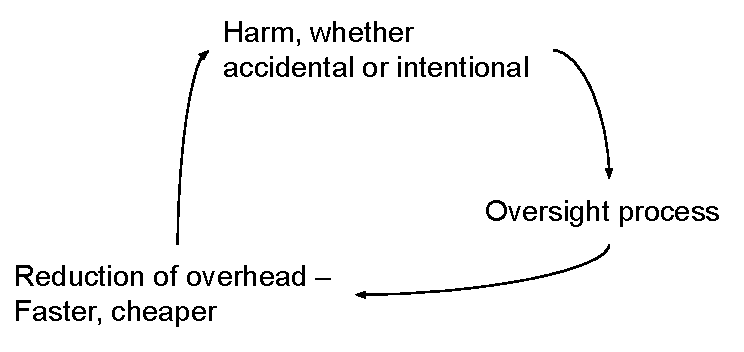
\includegraphics{images/process_loop_harm-oversight-improvement}
    \caption{loop: harm-oversight-improvement}
    \label{fig:harm-oversight-improvement}
\end{figure}



Bureaucracy is defined by processes.
As a counter force, social relationships.
Actually, processes are social relationships formalized

Processes are not consistent across people because the relationships vary


processes are about a defensible story for the bureaucrats involved -- not the actual equitable distribution



% https://graphthinking.blogspot.com/2021/04/laffer-curve-and-minimum-viable.html
social processes can work well for small tasks that are infrequent
social processes can be effective in anomalous situations
bureaucratic processes are useful under typical conditions

When no process exists, only people with relationships succeed. Processes enable novices to an organization to contribute value and gain experience. 





Does a process exist?

% https://graphthinking.blogspot.com/2015/07/notes-on-bureaucracy-and-social-network.html
Do participants know about existing processes?

Processes can be undocumented. Then oral folklore is the mechanism. 

% process design trade-offs
Processes with fewer people and fewer steps can be quicker and use fewer resources, but they are more fragile and less representative. Having more people involved helps with edge cases, but slows down the process. 


